

\section{Introduction}
% The very first letter is a 2 line initial drop letter followed
% by the rest of the first word in caps.
% 
% form to use if the first word consists of a single letter:
% \IEEEPARstart{A}{demo} file is ....
% 
% form to use if you need the single drop letter followed by
% normal text (unknown if ever used by IEEE):
% \IEEEPARstart{A}{}demo file is ....
% 
% Some journals put the first two words in caps:
% \IEEEPARstart{T}{his demo} file is ....
% 
% Here we have the typical use of a "T" for an initial drop letter
% and "HIS" in caps to complete the first word.
\IEEEPARstart{A}{ well-designed} graph is a powerful tool 
that transends barriers of language to
communicate complex concepts from author to audience. It becomes a 
problem if readers are unable to easily extract the main message, especially
when distortion is encoded. The source of a distortion may be due to 
intrinsic deformities in the graph or simply the perceptual limitations of
the audience. Examples include Tufte's \emph{Lie-Factor} \citep[p. 57--69]{tufte} in which the proportion of the physical space occupied by the graphic is 
inconsistent with underlying data; calculated ratio (of proportions) less than one indicate 
underrepresentation. Another example is the M\"{u}ller-Lyer family of illusions such as the sine wave, where viewers perceive extents at the curves to be of different height than in the straight regions even though all regions were of the same height \citep{day:1991}.

Regardless of the cause of distortion, the graph author has a duty to create visualizations that
 allows readers to extract an accurate interpretation of the underlying data. The \emph{Lie-Factor}
provides a quantitative method to evaluate distortion due to graph deformities. In order to ascertain the
impact of distortion due to perceptual limits, usability studies provide empirical evidence supporting 
underlying metaphorical models both known and unpredicted. We describe how a routine user study 
during development of parallel coordinates for categorical data led to the unexpected and unpredicted discovery of the \emph{line-width} illusion. We introduce the {\it common-angle plot} as an alternative  method for displaying categorical data in a manner that minimizes the effect from perceptual illusions.
The display preserves properties of parallel coordinates, such as the potential to visualize a large number of dimensions simultaneously, but also presents frequency information. Finally, we present results from user studies as evidence that common angle plots resolve the problem of the line width illusion. 
% You must have at least 2 lines in the paragraph with the drop letter
% (should never be an issue)

\section{Related Work}
This section describes a selection of related work as context for the contributions 
presented here.

\subsection{Line width illusion}

An example of the  {\it line width illusion} is displayed in  figure  \ref{playfair}. 


\begin{figure}
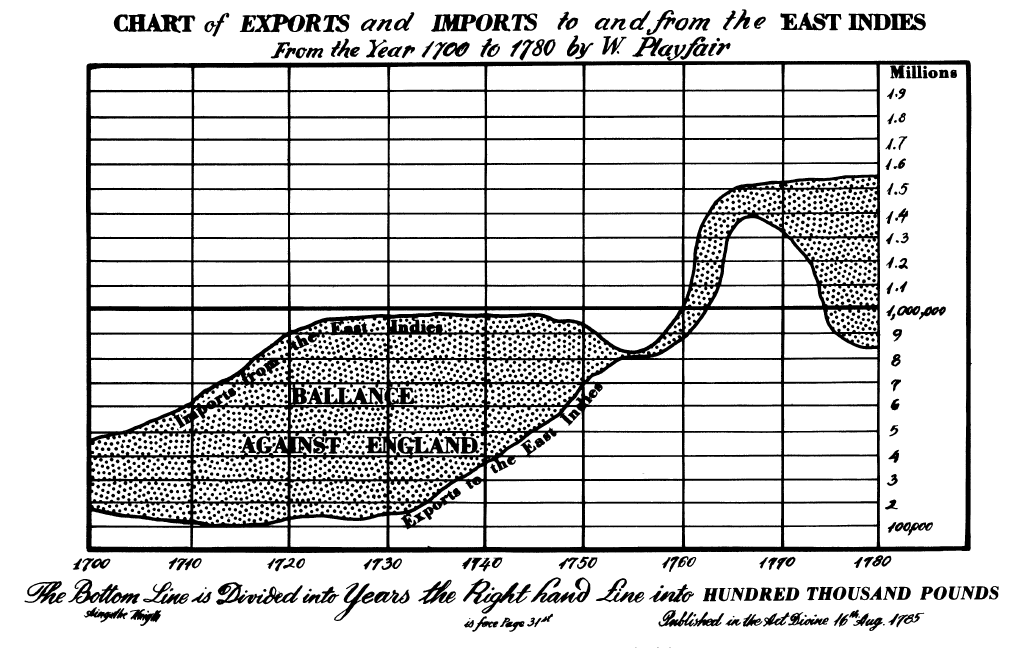
\includegraphics[width=.9\linewidth]{images/playfair_east_indies_gross}
\caption{\label{playfair}
Playfair's chart from the Commercial and Political Atlas (1786) showing the balance of trade between England and the East Indies.  In which years was the difference between imports and exports the highest? }
\end{figure}
This chart displays the balance of trade between England and the East Indies as shown by William Playfair in his Commercial and Political Atlas, 1786 \cite{playfair, playfair2}.  One purpose of this chart is to demonstrate the difference between imports and exports in a particular year and its pattern over that time frame. The difference in exports and imports is encoded as the vertical difference between the lines. When observers are asked to sketch out the difference between exports and imports  \citep{cleveland:1984}, they very often  miss the steep rise in the difference between the lines in the years between about 1755 and 1765. Figure \ref{playfair2} shows the  actual difference between imports and exports. 



\begin{figure}
\centering
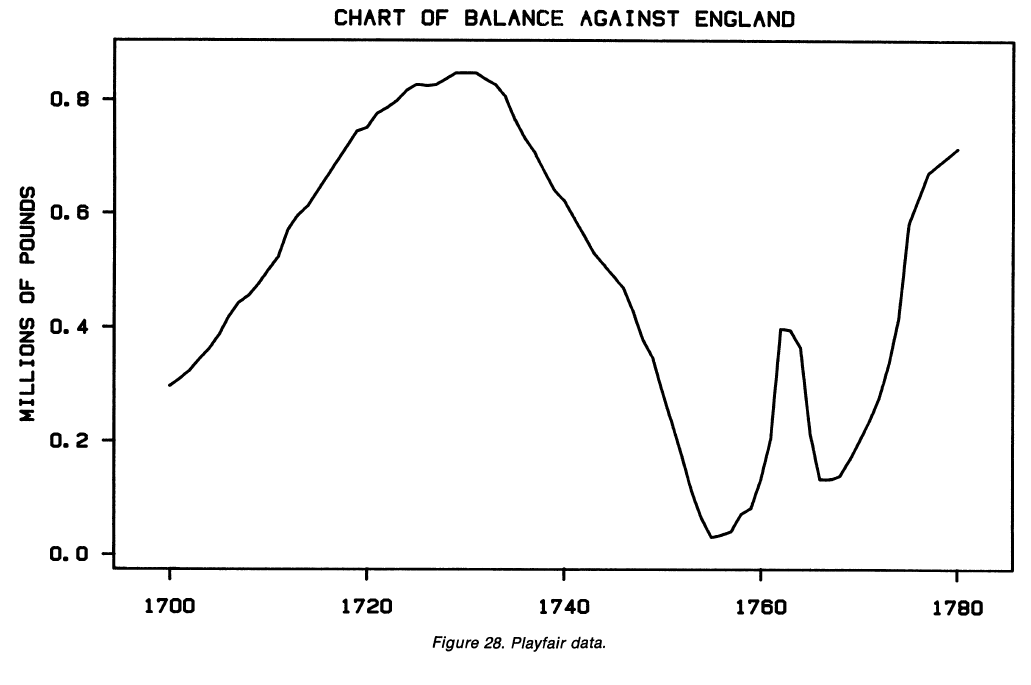
\includegraphics[width=.8\linewidth, height=.4\linewidth]{images/playfair_differenz_cleveland}
\caption{\label{playfair2}
Difference between exports and imports from England to and from the East Indies in the 18th century -- the steep rise in the difference around 1760  comes as a surprise to many viewers of the raw data in figure \ref{playfair}.  }
\end{figure}


This phenomenon  is known and widely discussed in statistical graphics literature \citep{cleveland:1984, tufte, wainer:2000, robbins:2005}. It  is due to our  tendency to assess distance between curves as the minimal (orthogonal) distance rather than the  vertical distance -- see sketch \ref{fig:linewidth} for a visual representation of both.


In the perception literature, this phenomenon is known as part of a group of geometrical optical misperceptions of a context-sensitive nature classified as M\"uller-Lyer illusions \citep{day:1991}. Interestingly, there seems to be a general agreement that this illusion exists, but a quantification of it is curiously absent from the literature. 

While we see the type of chart as shown in figure~\ref{playfair} proposed by Playfair quite commonly, particular in election years -- where these kind of charts are used to enable comparisons of support for several candidates, the recommendation from the literature is to avoid charts in which the audience is asked to do visual subtractions, and show these differences directly.

However, the line width illusion is not restricted to this situation only. We next discuss how other charts, such as the parallel sets plots \citep{kosara:2006}, are affected by it.


\subsection{Hammock plots}
\subsection{Strength of the line width illusion}
\subsection{Parallel sets}


% An example of a floating figure using the graphicx package.
% Note that \label must occur AFTER (or within) \caption.
% For figures, \caption should occur after the \includegraphics.
% Note that IEEEtran v1.7 and later has special internal code that
% is designed to preserve the operation of \label within \caption
% even when the captionsoff option is in effect. However, because
% of issues like this, it may be the safest practice to put all your
% \label just after \caption rather than within \caption{}.
%
% Reminder: the "draftcls" or "draftclsnofoot", not "draft", class
% option should be used if it is desired that the figures are to be
% displayed while in draft mode.
%
%\begin{figure}[!t]
%\centering
%\includegraphics[width=2.5in]{myfigure}
% where an .eps filename suffix will be assumed under latex, 
% and a .pdf suffix will be assumed for pdflatex; or what has been declared
% via \DeclareGraphicsExtensions.
%\caption{Simulation Results.}
%\label{fig_sim}
%\end{figure}

% Note that IEEE typically puts floats only at the top, even when this
% results in a large percentage of a column being occupied by floats.


% An example of a double column floating figure using two subfigures.
% (The subfig.sty package must be loaded for this to work.)
% The subfigure \label commands are set within each subfloat command,
% and the \label for the overall figure must come after \caption.
% \hfil is used as a separator to get equal spacing.
% Watch out that the combined width of all the subfigures on a 
% line do not exceed the text width or a line break will occur.
%
%\begin{figure*}[!t]
%\centering
%\subfloat[Case I]{\includegraphics[width=2.5in]{box}%
%\label{fig_first_case}}
%\hfil
%\subfloat[Case II]{\includegraphics[width=2.5in]{box}%
%\label{fig_second_case}}
%\caption{Simulation results.}
%\label{fig_sim}
%\end{figure*}
%
% Note that often IEEE papers with subfigures do not employ subfigure
% captions (using the optional argument to \subfloat[]), but instead will
% reference/describe all of them (a), (b), etc., within the main caption.


% An example of a floating table. Note that, for IEEE style tables, the 
% \caption command should come BEFORE the table. Table text will default to
% \footnotesize as IEEE normally uses this smaller font for tables.
% The \label must come after \caption as always.
%
%\begin{table}[!t]
%% increase table row spacing, adjust to taste
%\renewcommand{\arraystretch}{1.3}
% if using array.sty, it might be a good idea to tweak the value of
% \extrarowheight as needed to properly center the text within the cells
%\caption{An Example of a Table}
%\label{table_example}
%\centering
%% Some packages, such as MDW tools, offer better commands for making tables
%% than the plain LaTeX2e tabular which is used here.
%\begin{tabular}{|c||c|}
%\hline
%One & Two\\
%\hline
%Three & Four\\
%\hline
%\end{tabular}
%\end{table}


% Note that IEEE does not put floats in the very first column - or typically
% anywhere on the first page for that matter. Also, in-text middle ("here")
% positioning is not used. Most IEEE journals use top floats exclusively.
% Note that, LaTeX2e, unlike IEEE journals, places footnotes above bottom
% floats. This can be corrected via the \fnbelowfloat command of the
% stfloats package.



\section{Conclusion}
The conclusion goes here.





% if have a single appendix:
%\appendix[Proof of the Zonklar Equations]
% or
%\appendix  % for no appendix heading
% do not use \section anymore after \appendix, only \section*
% is possibly needed

% use appendices with more than one appendix
% then use \section to start each appendix
% you must declare a \section before using any
% \subsection or using \label (\appendices by itself
% starts a section numbered zero.)
%


\appendices
%\section{Proof of the First Zonklar Equation}
%Appendix one text goes here.
%
%% you can choose not to have a title for an appendix
%% if you want by leaving the argument blank
%\section{}
%Appendix two text goes here.


% use section* for acknowledgement
\section*{Acknowledgment}


The survey for this study was carried out with approval from  IRB-ID 12-204.


% Can use something like this to put references on a page
% by themselves when using endfloat and the captionsoff option.
\ifCLASSOPTIONcaptionsoff
  \newpage
\fi



% trigger a \newpage just before the given reference
% number - used to balance the columns on the last page
% adjust value as needed - may need to be readjusted if
% the document is modified later
%\IEEEtriggeratref{8}
% The "triggered" command can be changed if desired:
%\IEEEtriggercmd{\enlargethispage{-5in}}
